\chapter{Funktionsgruppen der Power-on-Reset-Schaltung}\label{chap:Schaltung}
Um eine zuverlässige Initialisierung des Chips zu erfüllen, wurde eine aus mehreren funktionalen Blöcken bestehende \gls{por}-Schaltung aufgebaut. Jede dieser Funktionsgruppen übernimmt eine spezifische Aufgabe innerhalb der Gesamtschaltung und trägt zur korrekten Erzeugung und Freigabe des Reset-Signals bei. Die wesentlichen Funktionsblöcke umfassen die Generierung einer Referenzspannung, eine zuverlässige Vergleichsschaltung, eine zeitgesteuerte Verzögerung zur sicheren Initialisierung sowie eine Schmitt-Trigger-Stufe zur Verbesserung der Störfestigkeit. 

Durch die modulare Aufteilung kann jeder dieser Blöcke gezielt auf die Anforderungen des analogen oder digitalen Teils des Chips angepasst werden. In den folgenden Abschnitten werden diese detailliert beschrieben und ihr Beitrag zur Gesamtschaltung erläutert (Kapitel 3.1 - 3.4). Anschließend wird dargelegt, welche Anpassungen für den Komparator des Digitalteils notwendig waren (Kapitel 3.5). 


\section{Komparator}
Ein entscheidendes Bauteil der \gls{por}-Schaltung ist der Komparator, da dieser bestimmt, wann das Reset-Signal aktiviert oder deaktiviert wird. Für die Realisierung des Komparators (siehe \autoref{fig:komparator}), werden \gls{cmos}-Transistoren verwendet. Hauptbestandteil dieser Schaltung ist das differenzielle Paar \gls{nmos}-Transistoren ($N_1$ und $N_2$), die an ihren Gates die Eingangssignale ($V_{inn}$ und $V_{inp}$) vergleichen. Dieses Paar bestimmt, welcher Transistor mehr Strom leitet, in Abhängigkeit von der Spannungsdifferenz zwischen $V_{inn}$ und $V_{inp}$~\cite{DesignOfAnalogCMOSIntegratedCircuits}. Der darüber liegende Stromspiegel, bestehend aus zwei \gls{pmos}-Transistoren ($P_0$ und $P_1$) und sorgt dafür, dass der gleiche Strom durch beide Seiten des Differenzverstärkers fließt. Damit wird sichergestellt, dass die Schaltung symmetrisch arbeitet. Für eine konstante Stromversorgung ist der \gls{nmos}-Transistor $N_3$ zuständig, der sich unter dem Differenzpaar $N_1$ und $N_2$ befindet \cite{ADofIntegratedCircuits}. 
%\vspace{1.5\baselineskip}
\begin{figure}[H]
    \begin{center}
        \begin{circuitikz}
            \ctikzset{tripoles/mos style/arrows}[line width=thick]
            \draw % Transformatoren 
            (3,0) node[pmos, emptycircle](pmosR){$P_2$}
            (-3,0) node[pmos, emptycircle, yscale=-1, rotate=180](pmosL){} 
                node at (pmosL.center) [anchor=center, xshift=-10pt] {$P_1$}
            
            (-3,-3) node[nmos, emptycircle](nmosL){$N_1$}
            (3,-3) node[nmos, emptycircle, yscale=-1, rotate=180](nmosR){}
                node at (nmosR.center) [anchor=center, xshift=-10pt] {$N_2$}
    
            (0,-5) node[nmos, emptycircle](nmos){$N_3$}
    
            % Verbindung zwischen Transformatoren
            (pmosR.drain) -- (nmosR.drain){}
                coordinate[pos=0.5](crosspointRR) % Mittelpunk zwischen pmosR und nmosR
            (pmosL.drain) -- (nmosL.drain){}
                coordinate[pos=0.5](crosspointLL) % Mittelpunk zwischen pmosL und nmosL
            (nmosL.source) -- ++(0,-0.25) -- ++(3,0)
            (nmosR.source) -- ++(0,-0.25) -- ++(-3,0) coordinate(Ibias)
                (Ibias) node[circle, fill, inner sep=1.5pt]{}
            (Ibias) -- (nmos.drain)
            
            (pmosL.source) -- ++(0,0.5) coordinate (tmp1) 
                -- ++(6,0) coordinate (tmp2) % rechte obere Koordinate
                -- (pmosR.source) coordinate (tmp3)
                (tmp1) -- (tmp2)
                    coordinate[pos=0.5](crosspointVdd)
                        (crosspointVdd) -- ++(0,0.5) coordinate(VDD)
                            node[above] {$V_{DD}$} % Text zwische Koordinate 1 und 2
                        (VDD) -- ++(-0.5,0)
                        (VDD) -- ++(0.5,0)
    
            (pmosL.gate) -- (pmosR.gate){}
                coordinate[pos=0.5](crosspointLR) % Mittelpunk zwischen pmosL und pmosR
    
            % Knoten und Verbindungen 
            (crosspointLL) node[circle, fill, inner sep=1.5pt]{} % Knoten links
            (crosspointLR) node[circle, fill, inner sep=1.5pt]{} % Knoten mitte
            (crosspointLL) -| (crosspointLR){} % Verbindung zwischen linken und mittleren Knoten
            (crosspointRR) node[circle, fill, inner sep=1.5pt]{}
                (crosspointRR) -- ++(1.5,0)
                    node[pos=1, above right, xshift=-15pt]{$V_{out}$}
            
            % Verbindung nmos.gate
            (nmosL.gate) -- (-4.5,-3)
                node[pos=0, above left]{$V_{inn}$}
            (nmosR.gate) -- (4.5,-3)
                node[pos=0, above right]{$V_{inp}$}
            (nmos.gate) -- (-1.5,-5)
                node[pos=0, above left]{$V_{ref}$}
    
            % Ground
            (nmos.source) 
                node [sground]{}
                node[right, xshift=5pt, yshift=-5pt]{Gnd}
            ;
    
        \end{circuitikz}
    \end{center}
    \caption[Aufbau Komparator für analogen Teil]{\\Quelle: Aufbau Komparator für analogen Teil (eigene Darstellung)}
    \label{fig:komparator}
\end{figure}
% \vspace{1.5\baselineskip}
Wenn die Spannung $V_{inn}$, die am Gate $N_1$ anliegt, größer ist als die Spannung $N_2$, dann wird $V_{inn}$ nach oben über den Stromspiegel zu $V_{out}$ geleitet. Ist $V_{inp}$ größer als $V_{inn}$, fließt der Strom direkt zu $V_{out}$ und nicht über den Stromspiegel. 

\section{Referenzspannung}
Damit ein zuverlässiges Reset-Signal generiert werden kann, wird eine Referenzspannung ($V_{ref}$) benötigt, die als Vergleichswert für die Schaltpunkte des Komparators dient. Für die Generierung von $V_{ref}$ sowie den Schaltpunkten des Komparators wird die Schaltung~(siehe \autoref{fig:Vref_old}) entworfen, welche sich wiederum in einzelne Funktionsblöcke unterteilen lässt. Der erste Funktionsblock ist die Generierung der Referenzspannung mittels Widerstandsteiler. Dieser besteht aus dem Widerstand~($R_0$) und \gls{nmos}-Transistor~($N_0$), wobei der Wert von $V_{ref}$ abhängig von der Dimensionierung von $R_0$ und $N_0$ ist. Ein weiterer entscheidender Bestandteil der Schaltung ist der Spannungsteiler, bestehend aus den Widerständen $R_1$,$R_2$ und $R_3$. Durch die gezielte Wahl der Widerstandswerte lassen sich die Schaltschwellen der \gls{cmos}-Transistoren festlegen, sodass diese bei bestimmten Spannungswerten umschalten. 
%\vspace{1.5\baselineskip}
\begin{figure}[H]
    \begin{center}
        \begin{circuitikz}[european]
            \ctikzset{tripoles/mos style/arrows}[line width=thick, european]
            % Widerstand
            \draw (-3,5) coordinate(resistor-begin) to[resistor, l={$R_0$}] (-3,0.5) coordinate(resistor-end);

            \draw (resistor-begin) node[circle, fill, inner sep=1.5pt]{};
            
            % NMOS Transistor
            \draw (-3,-0.5) node[nmos, anchor=drain] (nmosL) {$N_0$};

            % Verbindung von Drain des NMOS mit Widerstand
            \draw (resistor-end) -- (nmosL.drain);
            \draw (nmosL.gate) -- ++(-0.25,0) |- (resistor-end)
                node[circle, fill, inner sep=1.5pt]{}
                node[above, midway]{$V_{ref}$};
            %
            %*************************************************************************
            %
            % Widerstand R
            \draw (0,5) coordinate (resistor-begin1) to[resistor, l={$R_1$}] (0,2) coordinate (resistor-end1);
            \draw (0,2) coordinate (resistor-begin2) to[resistor, l={$R_2$}] (0,-1) coordinate (resistor-end2);
            \draw (0,-1) coordinate (resistor-begin3) to[resistor, l={$R_3$}] (0,-4) coordinate (resistor-end3);

            % NMOSR 
            \draw (3,2) node[nmos, rotate=270] (nmosR1) {}
                node at (nmosR1.center) [anchor=center, yshift=-10pt] {$N_1$}
                (nmosR1.source) -- (resistor-end1) % Verbinung zu Wiederständen 
                node[circle, fill, inner sep=1.5pt]{}; % Punkt am Ende der Verbindung 
            \draw (3,-1) node[nmos, rotate=270] (nmosR2) {}
                node at (nmosR2.center) [anchor=center, yshift=-10pt] {$N_2$}
                (nmosR2.source) -- (resistor-end2)
                node[circle, fill, inner sep=1.5pt]{};

            % NMOS Drain Verbindung
            \draw (nmosR1.drain) -- ++ (0.25,0) % horizontal nach rechts
                -- ++ (0,-3) coordinate (comp) % vertikale Linie 
                node[circle, fill, inner sep=1.5pt]{};

            \draw (nmosR1.gate) -- ++(0,0.25) -- ++(-0.75,0) 
                node[above, midway]{$V_{res}$};
            \draw (nmosR2.gate) -- ++(0,0.25) -- ++(-0.75,0)
                node[above, midway]{$V_{res0}$};

            % Dreieck am Ende von Vcomp
            \draw (6.75,-0.51) node[op amp] (triangle){}
                (triangle.+) -- (nmosR2.drain);
            \draw (triangle) node[above, yshift=27pt] {Komparator};  

            \draw (triangle.-) -- ++(-0.5,0) node[above]{$V_{ref}$};

            % Verbindung Ground
            \draw (nmosL.source) |- (resistor-end3)
                node[circle, fill, inner sep=1.5pt]{}
                -- ++(0,-0.25) node[sground]{}
                node[right, xshift=5pt, yshift=-5pt]{Gnd};     

            % Verbindung VDD
            \draw (resistor-begin1) -- ++(-3.73,0)
                node[above] {$V_{DD}$};

            % Arrow 
            \draw[->, thick, shorten >=10pt, shorten <=10pt, >=stealth] (resistor-end1) to[out=225,in=135] (resistor-end3)
                node[midway, left, xshift=-35pt, yshift=-10pt]{$V_{DD1}$};
                
            \draw[->, thick, shorten >=10pt, shorten <=10pt, >=stealth] (resistor-end2) to[out=-25,in=25] (resistor-end3)
                node[right,xshift=20pt, yshift=50pt]{$V_{DD2}$};
        \end{circuitikz}
    \end{center}
    \caption[Generierung des Referenzstrom durch Widerstand]{\\Quelle: Generierung des Referenzstrom durch Widerstand (Eigene Darstellung)}
    \label{fig:Vref_old}
\end{figure}
%\vspace{1.5\baselineskip}
Die Transistoren $N_1$ und $N_2$ werden mit den Signalen $V_{res}$ und $V_{res0}$ gesteuert. Außerdem verbinden $N_1$ und $N_2$ die Spannung $V_{DD1}$ und $V_{DD2}$ mit dem positiven Eingang des Komparators. Diese \gls{cmos}-Schalter sorgen somit für eine gezielte Modifikation der Vergleichsspannung, die dem Komparator zugeführt wird. Der Komparatorausgang wird durch eine nachgestellte Inverter-Kette verarbeitet, die als Buffer dienen und die Ausgangssignale $V_{res}$ und $V_{res0}$ zur Verfügung stellen. Somit wird bei inaktiven Reset-Signal ($V_{comp} = 0$) die höhere Spannung ($V_{DD1}$) als Vergleichsspannung verwendet, wodurch die höhere Schwellspannung $V_H$ (siehe \autoref{fig:Schwellspannung}) erzeugt wird. Im Gegensatz dazu wird bei einem aktiven Resest-Signal ($V_{comp} = 1$) die niedrigere Spannung $V_{DD2}$ verwendet, sodass eine geringere Reset-Spannung ($V_L$) (siehe \autoref{fig:Reset-Spannung}) realisiert wird.
\cite{DesignOfAnalogCMOSIntegratedCircuits}\cite{MicroelectronicCircuits}.

\section{Verzögerung des Reset}
Bei einer \gls{por}-Schaltung muss sichergestellt werden, dass der Reset-Zustand so lange aufrechterhalten wird, bis die Versorgungsspannung stabil ist. Gleichzeitig muss das System bei einem plötzlichen Spannungsabfall schnell in den Reset-Zustand zurückkehren, um Fehlfunktionen zu vermeiden. In diesem Schaltungsteil (siehe \autoref{fig:Delay}) der \gls{por}-Schaltung, wird die verzögerte Aktivierung beim Hochfahren als auch eine schnelle Reaktion beim Abfallen der Versorgungsspannung realisiert.
%\vspace{1.5\baselineskip}
\begin{figure}[H]
    \begin{center}
        \begin{circuitikz}[european]
            \ctikzset{tripoles/mos style/arrows}[line width=thick, european]
            
            % Transistoren links
            \draw (-4,0) node[pmos, emptycircle, yscale=-1, rotate=180](pmosL){}
                node at (pmosL.center) [anchor=center, xshift=-10pt]{$P_0$}
                (-4,-3) node[nmos](nmosL){$N_0$};
                
            % Transistoren rechts
            \draw (0,0) node[pmos, emptycircle](pmosR1){$P_1$}
                (0,-3) node[pmos, emptycircle](pmosR2){$P_2$}
                (0,-6) node[nmos](nmosR){$N_1$};
                
            % Verbindungen Transistroen links
            \draw (pmosL.drain) -- (nmosL.drain) 
                coordinate[pos=0.5](crosspointLL) % Mitte links
                (crosspointLL) node[circle, fill, inner sep=1.5pt]{}; % Verzweigung links 
                
            % Verbindung pmos gate
            \draw (pmosL.gate) -- (pmosR1.gate)
                coordinate[pos=0.5](crosspointPP)
                (crosspointPP) node[circle, fill, inner sep=1.5pt]{};
            \draw (nmosL.gate) -- ++(-.5,0)
                node[above]{$V_{gate}$}
                (nmosL.source) node[sground]{}
                node[right, xshift=5pt, yshift=-5pt]{Gnd};
                
            % Kurzschluss 
            \draw (crosspointLL) -| (crosspointPP);

            % VDD
            \draw (pmosL.source) -- ++(0,0.5) 
                node[circle, fill, inner sep=1.5pt]{};
            \draw (pmosR1.source) -- ++(0,0.5) -- ++(-5.475,0) 
                node[above]{$V_{DD}$};
                
                
            % Verbindungen rechts    
            \draw (pmosR1.drain) -- (pmosR2.source)
                (pmosR2.drain) -- (nmosR.drain)
                    coordinate[pos=0.5](crosspointRR) % Mittelpunkte rechts
                    (crosspointRR) node[circle, fill, inner sep=1.5pt]{}
                (nmosR.source) -- ++(2,0) coordinate[](nmosC)
                (nmosC) node[circle, fill, inner sep=1.5pt]{};
                
            % Gate rechts
            \draw (pmosR2.gate) -- ++(-0.5,0)
                    -- ++(0,-3) node[circle, fill, inner sep=1.5pt]{}
                (nmosR.gate) -- ++(-4.5,0) 
                    node[above]{$V_{comp}$};
                    
            % Kondensator 
            \draw (2,-4.5) node[circle, fill, inner sep=1.5pt]{}
                (2,-4.5) to[C, l={$C$}] (2,-6.5) -- (nmosC)
                (nmosC) -- ++(0,-0.25) node[sground]{}
                node[right, xshift=5pt, yshift=-5pt]{Gnd};
            \draw (crosspointRR) -- ++(4,0)
                node[above]{$V_{schmitt}$};
                
        \end{circuitikz}
    \end{center}
    \caption[Verzögerungselement]{\\Quelle: Verzögerungselement (eigene Darstellung)}
    \label{fig:Delay}
\end{figure}
% \vspace{1.5\baselineskip}
Zentraler Bestandteil dieses Schaltungsabschnitts ist der Stromspiegel, der aus zwei gekoppelten \gls{pmos}-Transistoren besteht. Der linke Transistor $P_0$ arbeitet als Referenzzweig, $P_1$ bildet den gespiegelten Zweig, der $^1/_5$ des Stroms führt, da die Kanalbreiten der \gls{pmos}-Transistoren ein Verhältnis von ${W_{P_0}}/{W_{P_1}} = \frac{1}{5}$ haben. Dieser Strom sorgt für die Ladung des Kondensators $C$ \cite{CircuitDesigLayoutAndSimulation}. Beim Anlegen der Versorgungsspannung ist der Kondensator zunächst ungeladen, und $V_{schmitt}$ bleibt auf 0. Der durch den Stromspiegel gelieferte Strom lädt $C$ langsam auf, weshalb die Spannungsänderung an $V_{schmitt}$ nur verzögert auftritt, was durch 
\begin{equation}
    i = C \frac{du}{dt}
\end{equation}
berechnet werden kann. Um den Ladevorgang zu verlängern, kann $C$ größer oder $I$ kleiner gewählt werden \cite{MicroelectronicCircuits}\cite{DesignOfAnalogCMOSIntegratedCircuits}. Wenn es einen Abfall von $V_{DD}$ gibt, soll so schnell wie möglich der Reset-Zustand wiederhergestellt werden. In diesem Fall wird der $N_1$ sofort leitend, wodurch sich der Kondenstor direkt über diesen Transistor nach Masse entlädt. Durch die hohe Elektronenbeweglichkeit im \gls{nmos}-Kanal wird $C$ im Vergleich zur Ladezeit sehr schnell entladen. Somit wird das Reset-Signal sofort ausgelöst und das System in einen definierten Startzustand zurückgesetzt \cite{ElectronicDevices}. 

\section{Schmitt-Trigger}
Ein Schmitt-Trigger ist eine spezielle Art von Komparator mit Hysterese, dieser erzeugt ein stabiles Ausgangssignal, indem kleinere Spannungsschwankungen oder Rauschen am Eingang ignoriert werden. Die Schaltung aus \autoref{fig:schmitt-trigger} besteht aus einer Kombination aus \gls{pmos}- und \gls{nmos}-Transistoren, die in einer invertierten Struktur miteinander verbunden sind. 
%\vspace{1.5\baselineskip}
\begin{figure}[H]
    \begin{center}
        \begin{circuitikz}
            \ctikzset{tripoles/mos style/arrows}[line width=thick]
            \draw % Transformatoren 
            (0,2.5) node[pmos, emptycircle](pmos1){$P_0$}
            (3,0.95) node[pmos, emptycircle](pmos2){$P_2$}
            (0,0) node[pmos, emptycircle](pmos3){$P_1$} 
            (0,-2) node[nmos](nmos1){$N_0$}
            (3,-2.95) node[nmos](nmos2){$N_2$}
            (0,-4.5) node[nmos](nmos3){$N_1$};
        
            %Verbindung zwischen Transistoren
            \draw (pmos1.drain) -- (pmos3.source); % Verbindung von pmos1 zu pmos3 (senkrecht)
            \draw (pmos2.source) -- (pmos1.drain) % Verbindung zu pmos2 
                node[circle, fill, inner sep=1.5pt] {}; % Punkt an Verbindung
            \draw (pmos3.drain) -- (nmos1.drain); % Verbindung von pmos3 zu nmos1 
            \draw (nmos1.source) -- (nmos3.drain); % Verbindung von nmos1 zu nmos3
            \draw (nmos2.source) -- (nmos3.drain) % Verbindung zu noms2 
                node[circle, fill, inner sep=1.5pt] {};
            \draw (nmos3.source) 
                node[sground] {}
                node[right, xshift=5pt, yshift=-5pt]{Gnd};
            \draw (pmos2.drain)
                node[sground,] {}
                node[right, xshift=5pt, yshift=-5pt]{Gnd}; % Ground an pmos2
            \draw (pmos2.gate) -- (nmos2.gate) 
                coordinate[pos=0.5](crosspoint); % Mittelpunkt der Verbindung 
            
            % Vin                           
            \draw (-2.5,-1) -- (-1.5,-1) coordinate (Vin)% Vin Linie (zu Gates)
                node[pos=0, above left, xshift=10pt] {$V_{in}$} % Beschriftung oberhalb der Linie
                node [circle, fill, inner sep=1.5pt] {};

            %Vin connections 
            \draw (5,-1) -- (0,-1) % Vout Linie
                node [pos=0, above right, xshift=-25pt] {$V_{out}$}
                node [circle, fill, inner sep=1.5pt] {};
            \draw (crosspoint) node[circle, fill, inner sep=1.5pt] {}; % Punkt an Kreuzung
            \draw % Verbindung der Gates
                (pmos1.gate) -- ++(-0.5,0) -- (Vin);
            \draw % Verbindung der Gates
                (nmos3.gate) -- ++(-0.5,0) -- (Vin);
            \draw % Verbindung der Gates
                (pmos3.gate) -- ++(-0.5,0) 
                node[circle, fill, inner sep=1.5pt] {};
            \draw % Verbindung der Gates
                (nmos1.gate) -- ++(-0.5,0) 
                node[circle, fill, inner sep=1.5pt] {};    

            % VDD 
            \draw (-0.5,3.5) -- (0.5,3.5) % VDD an pmos1
                node[midway, above] {$V_{DD}$} % Beschriftung oberhalb der Linie
                (0,3.5) -- (pmos1.source);
            \draw (2.5,-1.95) -- (3.5,-1.95) % VDD an nmos2
                node[midway, above] {$V_{DD}$} % Beschriftung oberhalb der Linie
                (3,-1.95) -- (nmos2.drain); 
                
        \end{circuitikz}
    \end{center}
    \caption[Aufbau Schmitt-Trigger]{\\Quelle: Eigene Darstellung Aufbau Schmitt-Trigger in Anlehnung an \cite[S. 524]{CircuitDesigLayoutAndSimulation}}
    \label{fig:schmitt-trigger}
\end{figure}
%\vspace{1.5\baselineskip}
Die Schaltschwellen des Komparators $V_H$ und $V_L$ (siehe \autoref{fig:ST_symbol}) können durch die Dimensionierung der Länge ($L$) und Weite ($W$) der Transistroen eingestellt werden \cite{CircuitDesigLayoutAndSimulation}\cite{S-Trigger_design}\cite{LowPowerS-Trigger}.  

\section{Gesamte PoR-Schaltung}
Nach einem Test der einzelnen Funktionsblöcke auf ihre jeweilige Funktionalität, wurden diese Blöcke zu einem Gesamtsystem (siehe \ref{fig:PoR_complete}) zusammengesetzt. Der erste vollständige Aufbau der \gls{por}-Schaltung erfolgte für den analogen Schaltungsteil, der mit einer Versorgungsspannung von 5 V betrieben wird. Es wurden Anpassungen vorgenommen, wobei besonders die Weite der Transistoren eine große Rolle spielte, um die Schaltschwellen und die Zeitverzögerung an die Anforderungen anzupassen. Nachdem die gesamte Funktion der Schaltung für den analogen Schaltungsteil durch einfache Simulationen bestätigt wurde, erfolgte eine Anpassung der Schaltung für den digitalen Teil des \gls{ic}. Der digitale Teil des Systems arbeitet mit einer deutlich niedrigeren Versorgungsspannung von 1.5 V, weshalb andere Transistoren verwendet werden mussten. Während die Grundstruktur der \gls{por}-Schaltung beibehalten wurde, war eine Überarbeitung des Komparators erforderlich, da dessen Ausgangssignal nicht wie erwartet funktionierte.

\subsection{Komparator für digitalen IC Teil}
Zur Lösung dieses Problems wurde der Komparator für den digitalen Teil gezielt angepasst. Die geringere Versorgungsspannung von 1.5 V führt dazu, dass der Komparator nicht mehr zuverlässig schaltet. Deswegen wurde ein \gls{ota} als Komparator (siehe \autoref{fig:komparator1.5}) implementiert, da dieser durch Verstärkung der Eingangsspannungsdynamik für eine bessere Schaltgenauigkeit sorgt \cite{CMOS_Analog_Circuit_Design}. 
%\vspace{1.5\baselineskip}
\begin{figure}[H]
    \begin{center}
        \begin{circuitikz}
            \ctikzset{tripoles/mos style/arrows}[line width=thick]
            \draw % Transformatoren 
            (1.5,0) node[pmos, emptycircle, yscale=-1, rotate=180](pmosR){}
                node at (pmosR.center) [anchor=center, xshift=-10pt] {$P_2$}
            (5,0) node[pmos, emptycircle](pmosR1){$P_3$}
            (-1.5,0) node[pmos, emptycircle](pmosL){$P_1$} 
            (-5,0) node[pmos, emptycircle, yscale=-1, rotate=180](pmosL1){}
                node at (pmosL1.center) [anchor=center, xshift=-10pt] {$P_0$}
            
            (-1.5,-3) node[nmos, emptycircle](nmosL){$N_0$}
            (-5,-6) node[nmos, emptycircle, yscale=-1, rotate=180](nmosL1){}
                node at (nmosL1.center) [anchor=center, xshift=-10pt] {$N_2$}
            (1.5,-3) node[nmos, emptycircle, yscale=-1, rotate=180](nmosR){}
                node at (nmosR.center) [anchor=center, xshift=-10pt] {$N_1$}
            (5,-6)node[nmos, emptycircle](nmosR1){$N_4$}
    
            (0,-6) node[nmos, emptycircle](nmos){$N_3$}
    
            % Verbindung zwischen Transformatoren
            (pmosR.drain) -- (nmosR.drain){}
                coordinate[pos=0.5](crosspointRR) % Mittelpunk zwischen pmosR und nmosR
            (pmosL.drain) -- (nmosL.drain){}
                coordinate[pos=0.5](crosspointLL) % Mittelpunk zwischen pmosL und nmosL
            (nmosL.source) -| (nmos.drain) |- (nmosR.source){}

            (pmosL1.drain) -- (nmosL1.drain){}
            (pmosR1.drain) -- (nmosR1.drain){}
                coordinate[pos=0.5](Vout)

            (pmosL1.gate) -- (pmosL.gate){}
                coordinate[pos=0.5](MPL)
            (pmosR1.gate) -- (pmosR.gate){}
                coordinate[pos=0.5](MPR)
            
            % Knoten und Verbindungen 
            (crosspointLL) node[circle, fill, inner sep=1.5pt]{} % Knoten links
            (crosspointRR) node[circle, fill, inner sep=1.5pt]{}
            (Vout) node[circle, fill, inner sep=1.5pt]{}
                (Vout) -- ++(1,0)
                    node[pos=0, above right, xshift=15pt]{$V_{out}$}
            (MPL) node[circle, fill, inner sep=1.5pt]{}
                (MPL) |- (crosspointLL) 
            (MPR) node[circle, fill, inner sep=1.5pt]{}
                (MPR) |- (crosspointRR)

            (0,-4.5) -- ++(-5,0)
                node[circle, fill, inner sep=1.5pt]{}
            (0,-4.5) -- ++(3.25,0) coordinate[pos=1](Rechts)
                (Rechts) |- (nmosR1.gate)

            (nmosL1.gate) -- ++(.77,0) -- ++(0,1.5) 
                node[circle, fill, inner sep=1.5pt]{}

            (nmosL1.source) -- ++(0,-0.25)
                coordinate(Lvss)  
            (nmosR1.source) -- ++(0,-0.25)
                coordinate(Rvss)
            (nmos.source) -- ++(0,-0.25)
                coordinate[pos=0.5](Source)
                    node[circle, fill, inner sep=1.5pt]{}
            (Lvss) -- (Rvss) 
                
            % Verbindung nmos.gate
            (nmosL.gate) -- ++(-.5,0)
                node[pos=0, above left]{$V_{inn}$}
            (nmosR.gate) -- ++(.5,0)
                node[pos=0, above right]{$V_{inp}$}
            (nmos.gate) -- ++(-.5,0)
                node[pos=0, above left]{$V_{ref}$}
    
            % Ground
            (Source) -- ++(0,-0.5)
                node [sground]{}
                node[right, xshift=5pt, yshift=-5pt]{Gnd}

            % Vdd connection 
            (pmosL1.source) -- ++ (0,0.25) 
                node[circle, fill, inner sep=1.5pt]{}
            (pmosL.source) -- ++ (0,0.25)
                node[circle, fill, inner sep=1.5pt]{}
            (pmosR.source) -- ++ (0,0.25)
                node[circle, fill, inner sep=1.5pt]{}
            (pmosR1.source) -- ++ (0,0.25) -- ++(-11,0)
                node[above ]{$V_{DD}$}
            ;
    
        \end{circuitikz}
    \end{center}
    \caption[Aufbau Komparator für digitalen Teil]{\\Quelle: Eigene Darstellung Aufbau Komparator für den digitalen Teil in Anlehnung an \cite[S. 1217]{opamp}}
    \label{fig:komparator1.5}
\end{figure}
% \vspace{1.5\baselineskip}
Diese \gls{ota}-Schaltung wird als Komparator genutzt, um eine Spannungsschwelle präzise zu detektieren und zu verstärken. $N_0$ und $N_0$ bilden wieder ein Differenzpaar für die Eingangsspannungen $V_{inn}$ und $V_{inp}$. Der Arbeitsstrom für das Differenzpaar wird von dem \gls{nmos}-Transistor $N_3$ möglichst konstant bereitgestellt. Die Transistoren $P_0$ und $P_1$ sowie $P_2$ und $P_3$ bilden jeweils einen Stromspiegel, der den Strom des Differenzpaars symmetrisch auf beide Arme verteilt. Dadurch verbessert sich der Aussteuerbereich der Ausgangsspannung~($V_{out}$). Der Transistor $N_2$ spiegelt den Strom zu dem Transistor $N_4$. Wenn der Drainstrom~($I_D$) von~$N_4$ größer als $I_D$ von $P_3$ ist, dann ist $V_{out} = 0$ V. Wenn der Drainstrom~{$I_D$} von~$N_4$ kleiner als~$I_D$ von~$P_3$ ist, dann ist $V_{out} = V_{DD}$. Diese Architektur wird als \enquote{Folded-Cascode-OTA} bezeichnet und dient zur präzisen Verstärkung von Differenzsignalen mit hoher Verstärkung~\cite{CMOS_Analog_Circuit_Design}\cite{DesignOfAnalogCMOSIntegratedCircuits}.

Neben den Anpassungen am Komparator wurden auch kleinere Optimierungen an der restlichen Schaltung für den digitalen Teil des \glspl{ic} vorgenommen. Diese betrafen insbesondere die Widerstandsnetzwerke zur Einstellung der Schaltschwellen sowie die Dimensionierung der Transistoren. Diese Anpassungen gewährleisten, dass die gesamte \gls{por}-Schaltung auch für den digitalen Bereich zuverlässig funktioniert. 

Nach Abschluss dieser Überarbeitungen wurden sowohl die analoge als auch die digitale Version der \gls{por}-Schaltung in ihrer Gesamtheit getestet. Die Funktionalität konnte in beiden Fällen bestätigt werden (siehe \autoref{fig:por_waveform}),
\begin{figure}[h]
    \centering
    \begin{tikzpicture}
        % Das Bild einfügen
        \node[anchor=south west, inner sep=0] (image) at (-1,0) 
              {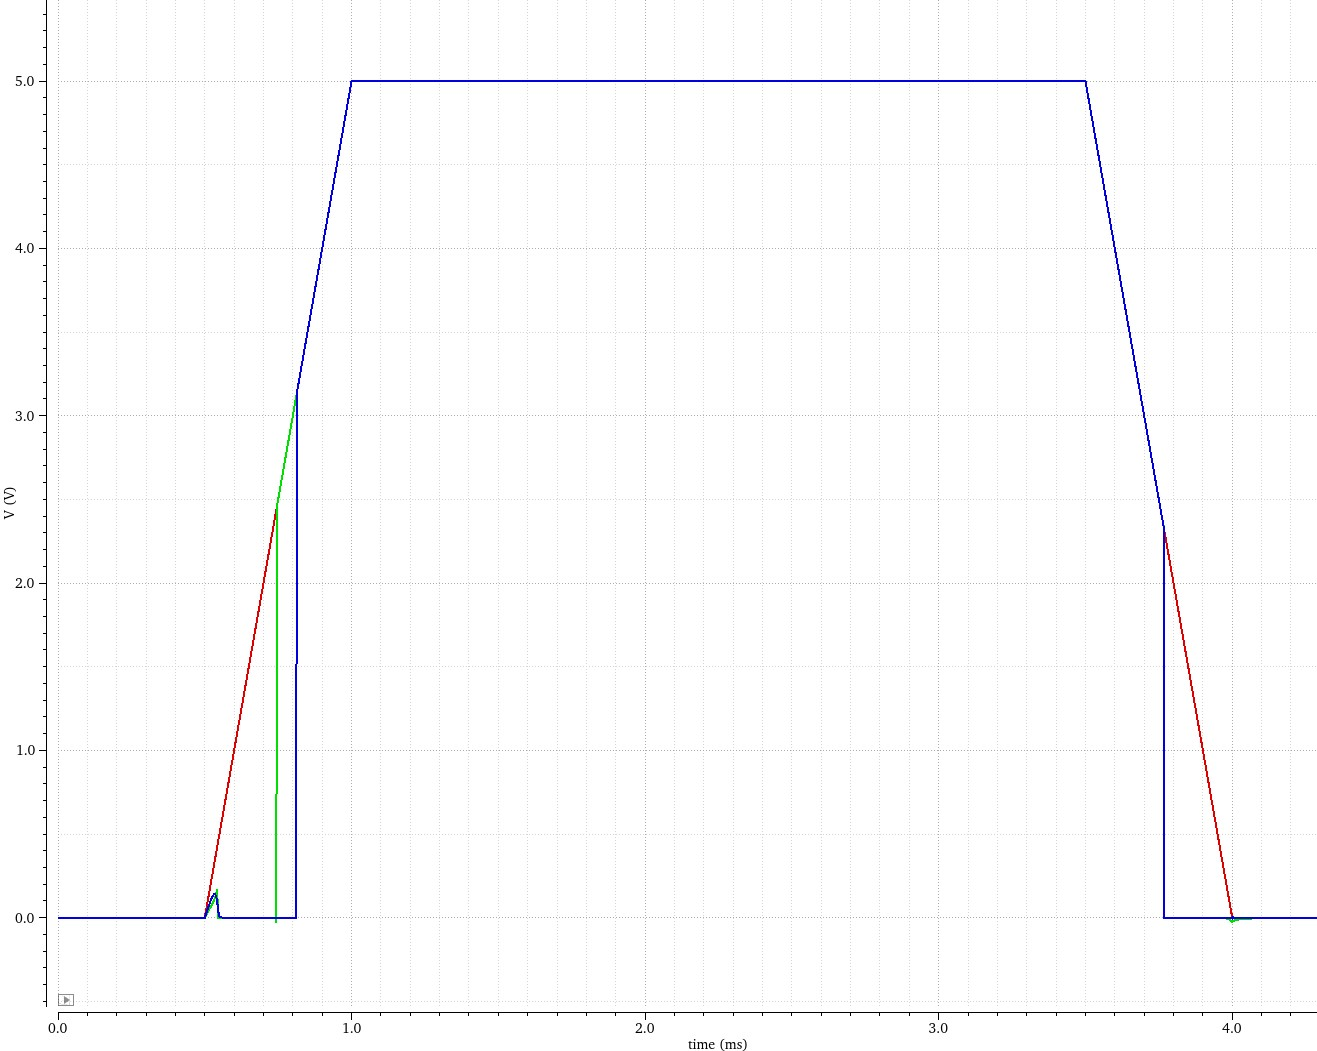
\includegraphics[width=0.8\textwidth]{figures/CD/waveform_standard.jpg}};

        % Legende hinzufügen
        \begin{scope}[shift={(0,-1)}]  % Position der Legende anpassen
            \draw[white] (0,0) rectangle (3.2,1.8); % Hintergrund für die Legende
            \node[anchor=west] at (-2,0.5) {\footnotesize\textcolor{red}{\textbf{---}} Betriebsspannung ($V_{DD}$)};
            \node[anchor=west] at (2,0.5) {\footnotesize\textcolor{green}{\textbf{---}} Komparatorausgang ($V_{comp}$)};
            \node[anchor=west] at (6.5,0.5) {\footnotesize\textcolor{blue}{\textbf{---}} Ausgang PoR-Schaltung ($V_{out}$)};
        \end{scope}
    \end{tikzpicture}
    \caption[Spannungsverläufe der Power-on-Reset-Schaltung]{: Spannungsverläufe der Power-on-Reset-Schaltung}
    \label{fig:por_waveform}
\end{figure}
 sodass beide Varianten nun so weiter optimiert werden können, um exakt den vorgegebenen Spezifikationen zu entsprechen. Dies umfasst unter anderem die präzise Abstimmung der Schaltschwellen sowie die Sicherstellung, dass die Reset-Signale unter allen Betriebsbedingungen rechtzeitig und zuverlässig zur Verfügung stehen. So wird sichergestellt, dass die \gls{por}-Schaltung sowohl im analogen als auch im digitalen Bereich ihre Aufgabe erfüllt und sich keine undefinierten Zustände im System einstellen. 